\subsection{Flexar coils}
Flexar coils are flexible PCB coils designed by the independent researcher \textbf{Carl Bugeja} \cite{Carl_Bugeja}.
He designed these very thin flexible coils intending to use them to actuate very \textbf{small robots} and \textbf{lightweight objects}.
This characteristic comes at the cost of not being able to produce very high magnetic fields.
We will be using for this research an old model of the Flexar coil that precedes the opening of the company \textbf{microbots} \cite{microbots}.
\begin{figure}[H]
    \centering
    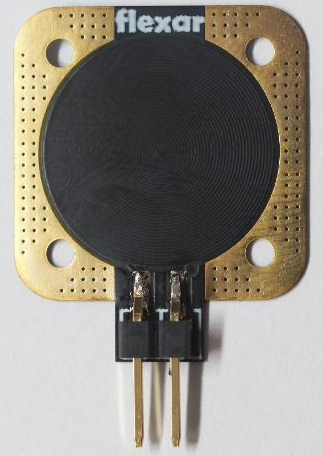
\includegraphics[width=0.4\linewidth]{Chapters/Chapter5/Coils_alternatives/Figures/Flexar_coil.png}
    \caption{Flexar coil }
    \label{fig:Flexar_coil}
\end{figure}


\subsubsection{Lower resistance and power needs}
We previously discussed the Flexar coil's characteristics in section \ref{subsec: Application challenges}.
But to sum up they have a resistance of about \textbf{30$\Omega$}, external radius of \textbf{$6.86\cdot10^{-3}$m}, internal one of about \textbf{$10^{-4}$m}, and number of spires equal to \textbf{70} (composed of two coils of 35 in series).

\begin{samepage}
    It can handle up to about \textbf{0.8W} before starting to release too much heat.
    \nopagebreak

    We report here the same graph as the previously cited section:
    \nopagebreak

    \begin{figure}[H]
        \centering
        \resizebox{0.5\textwidth}{!}{
            \begin{tikzpicture}
    \begin{axis}[
            xmin=0, ymin=0, xmax=8, ymax=2.5, samples=500,
            xlabel={Voltage [$V_{rms}$]},ylabel={Power [$W$]}, title={Power output vs $V_{rms}$}
        ]

        \addplot[blue, thick, domain=0:8, name path=func] (x, x^2/30);
        \addplot[red, thick, name path=limit] coordinates {
            (sqrt(0.8*30), \pgfkeysvalueof{/pgfplots/ymin}) 
            (sqrt(0.8*30), \pgfkeysvalueof{/pgfplots/ymax})
        }; % vertical limit line 

        \path[name path=axis] (axis cs:\pgfkeysvalueof{/pgfplots/xmin},0) -- (axis cs:\pgfkeysvalueof{/pgfplots/xmax},0);
        \path[name path=vend] (axis cs:\pgfkeysvalueof{/pgfplots/xmax},\pgfkeysvalueof{/pgfplots/ymin}) -- (axis cs:\pgfkeysvalueof{/pgfplots/xmax},\pgfkeysvalueof{/pgfplots/ymax});

        \addplot[red!25] fill between [of = limit and vend];
        % TODO: Add label to the limit line and legend
    \end{axis}
\end{tikzpicture}
        }
        \caption{Power profile of the Flexar coil}
        \label{fig: Flexar_heat_graph}
    \end{figure}
    \nopagebreak

    As we can see in figure \ref{fig: Flexar_heat_graph}, the Flexar coil can handle more power than the Dresden coil.
\end{samepage}

\subsubsection{Higher magnetic field strength}
Due to their characteristics, Flexar coils can produce \textbf{higher magnetic fields} than the Dresden coil but not unlike them, they are \textbf{still limited} by the power they can handle.
\begin{figure}[H]
    \centering
    \resizebox{0.5\textwidth}{!}{ 
        \begin{tikzpicture}
    \begin{axis}[
            xmin=0, ymin=0, xmax=1, ymax=8e-3, samples=500,
            xlabel={Voltage [$V_{rms}$]},ylabel={Magnetic Field [$T$]}, title={Magnetic Field vs $V_{rms}$}
        ]

        \addplot[blue, thick, domain=0:8, name path=func] (x, 0.005*x^0.5);
        \addplot[red, thick, name path=limit] coordinates {
            (0.8, \pgfkeysvalueof{/pgfplots/ymin}) 
            (0.8, \pgfkeysvalueof{/pgfplots/ymax})
        }; % vertical limit line 

        \path[name path=axis] (axis cs:\pgfkeysvalueof{/pgfplots/xmin},0) -- (axis cs:\pgfkeysvalueof{/pgfplots/xmax},0);
        \path[name path=vend] (axis cs:\pgfkeysvalueof{/pgfplots/xmax},\pgfkeysvalueof{/pgfplots/ymin}) -- (axis cs:\pgfkeysvalueof{/pgfplots/xmax},\pgfkeysvalueof{/pgfplots/ymax});

        \addplot[red!25] fill between [of = limit and vend];
        % TODO: Add label to the limit line and legend
    \end{axis}
\end{tikzpicture}
    }
    \caption{Magnetic field produced by the Flexar coil}
    \label{fig: Flexar_magnetic_field_vs_P}
\end{figure}

As we can observe in figure \ref{fig: Flexar_magnetic_field_vs_P}, the Flexar coil, at the power limit of the Dresden coil, can produce a \textbf{higher magnetic field} (in the order of \textbf{2.5mT}).
This proves that the Flexar coil is \textbf{more capable} than the Dresden coil in producing magnetic fields but even at its power limit, the field produced is \textbf{still feeble} (it is in the order of \textbf(\textbf{4mT})).

\subsubsection{Higher flexibility}
Flexible PCBs are made of a substrate of \textbf{polyimide}, which is a \textbf{very flexible material}.
It can withstand being bent at a very tight radius \textbf{multiple times without breaking}.

Between the layers of polyimide, we have the \textbf{copper traces} that don't require any tinning to work.
This makes the Flexar coil \textbf{more durable} than the Dresden coil, as it doesn't have any parts that can crack due to bending or heating and cooling.

Also, we observed that the Flexar coil can withstand temperatures in exceed of \textbf{100$^{\circ}$C}.

